\chapter{Introduzione}

La teoria che studieremo è una \textit{teoria geometrica}:

\textbf{I 5 postulati di Euclide:}
\begin{enumerate}
    \item Per due qualsiasi punti $A$ e $B$, esiste esattamente una retta che li attraversa.
    \item Una retta può essere prolungata indefinitamente in entrambe le direzioni.
    \item Dato un punto $O$ ed un raggio $R$, esiste esattamente un cerchio con centro in $O$ e raggio $R$.
    \item Tutti gli angoli retti sono congruenti.
    \item Data una retta $R$ ed un punto $P$ non appartenente a $R$, esiste esattamente una retta passante per $P$ che è parallela a $R$.
\end{enumerate}

Il quinto postulato è più complesso degli altri; nel corso del tempo, i matematici hanno provato più volte a dimostrare il quinto postulato basandosi sui restanti quattro. In seguito fu scoperto che il quinto è indipendente dagli altri.

\textbf{Conseguenze:}
\begin{enumerate}
    \item Non esiste alcuna retta parallela a $R$ passante per $P$ \\
    \quad $\rightarrow$ Geometrie ellittiche piane $[S^2]$
    \item Esistono due o più rette parallele a $R$ passanti per $P$ \\
    \quad $\rightarrow$ Geometrie iperboliche piane $[H^2]$
\end{enumerate}

\begin{figure}[H]
    \centering
    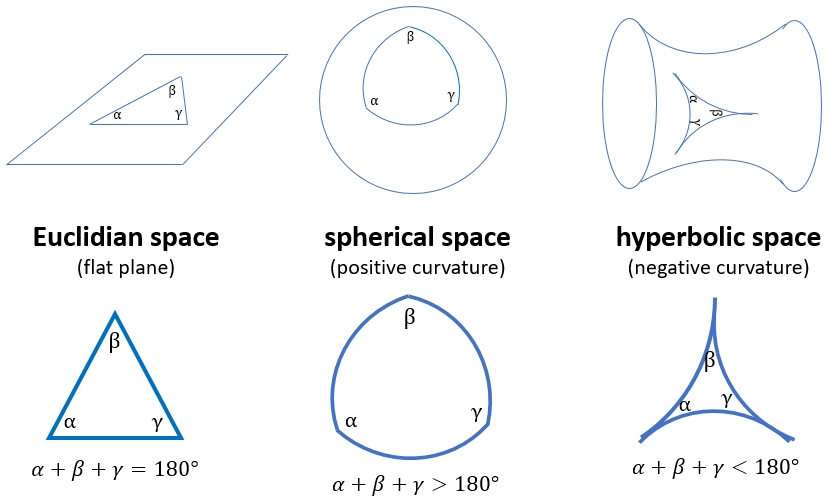
\includegraphics[width=0.5\textwidth]{assets/geometries.png}
    \caption{Geometrie ellittiche e iperboliche}
\end{figure}

\subsubsection{Geometria Ellittica}

La geometria ellittica piana è una forma di geometria non euclidea che rifiuta il quinto postulato di Euclide, il quale in geometria euclidea garantisce l'esistenza di una sola retta parallela passante per un dato punto. In geometria ellittica, non esistono rette parallele; invece, ogni coppia di rette si interseca eventualmente.

Un classico esempio è la geometria sferica, in cui le “rette” sono rappresentate da grandi cerchi su una sfera.

\begin{figure}[H]
    \centering
    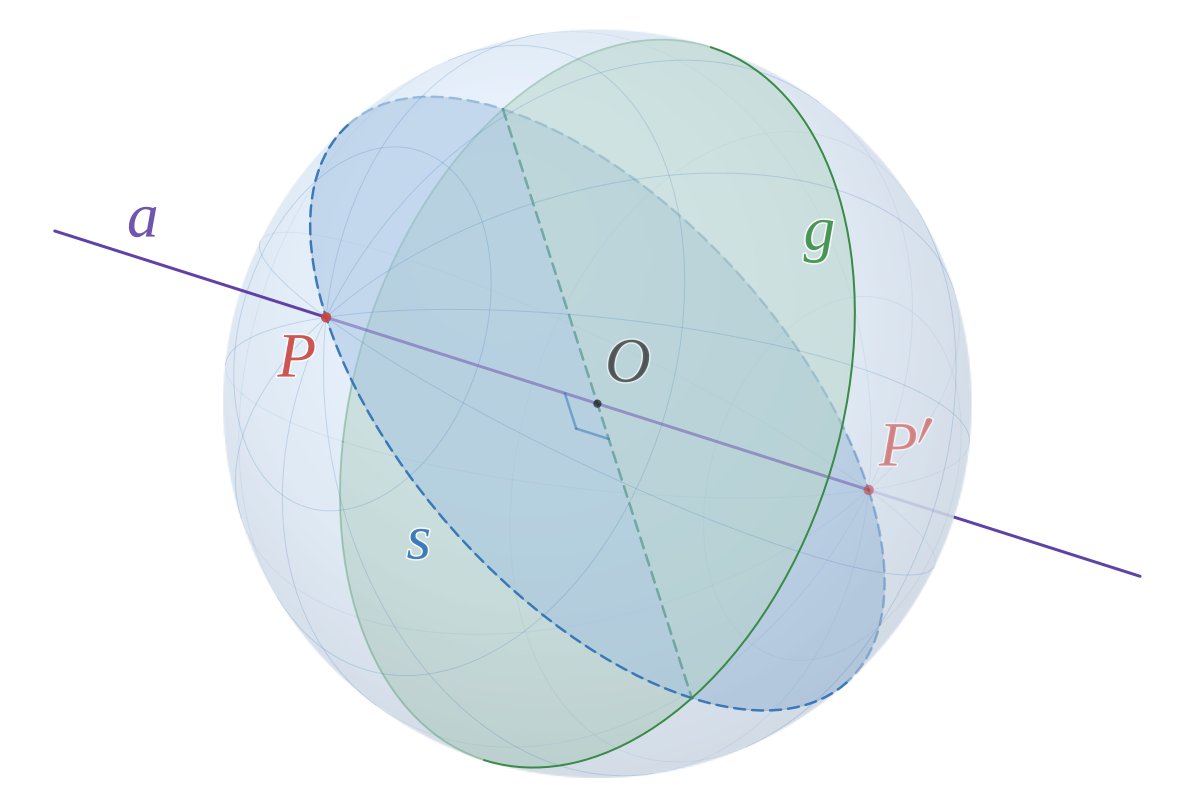
\includegraphics[width=0.5\textwidth]{assets/spherical_geometry.png}
    \caption{Geometria sferica}
\end{figure}

In questo contesto, i triangoli, noti come triangoli sferici, mostrano una proprietà intrigante: la somma dei loro angoli interni supera i 180° (un fenomeno noto come eccesso sferico), con l'eccesso proporzionale all'area del triangolo.

\begin{figure}[H]
    \centering
    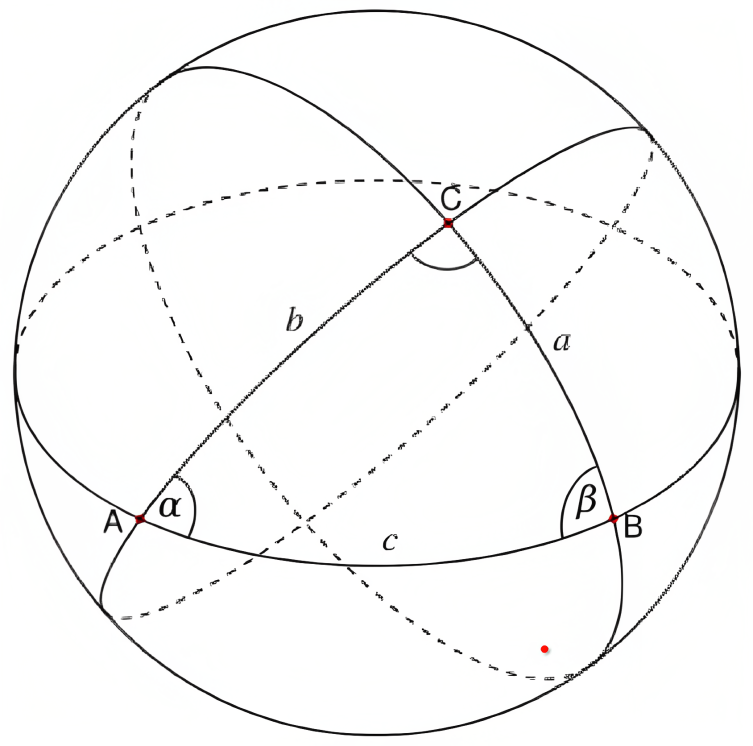
\includegraphics[width=0.5\textwidth]{assets/spherical_triangle.png}
    \caption{Triangolo sferico}
\end{figure}

\subsubsection{Geometria Iperbolica}

La geometria iperbolica piana è una forma di geometria non euclidea che rifiuta il quinto postulato di Euclide, il quale in geometria euclidea garantisce l'esistenza di una sola retta parallela passante per un dato punto. In geometria iperbolica, esistono molteplici rette parallele, e la somma degli angoli in un triangolo è sempre inferiore a 180°.

% \begin{figure}[H]
%     \centering
%     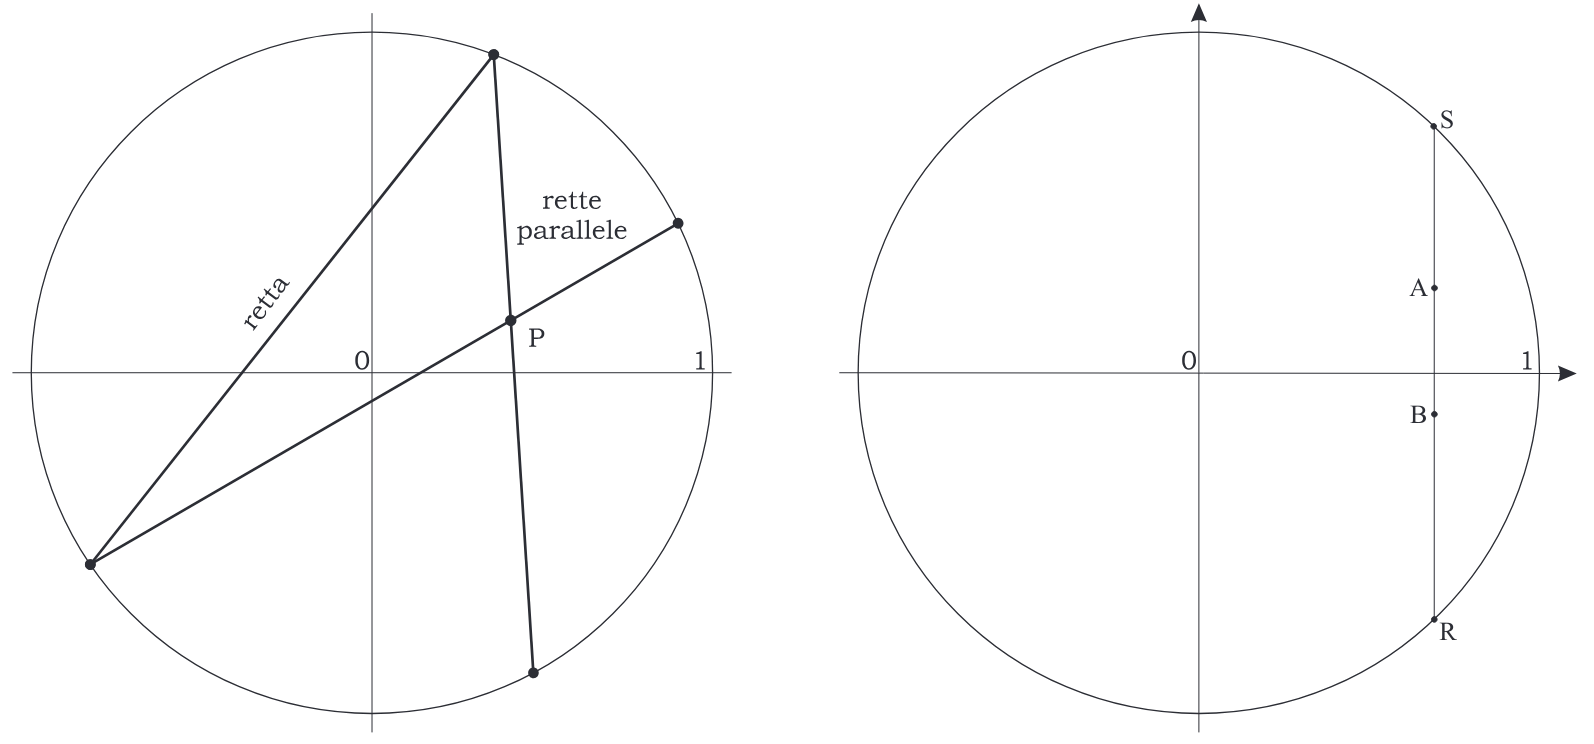
\includegraphics[width=0.5\textwidth]{assets/hyperbolic_geometry.png}
%     \caption{Geometria iperbolica}
% \end{figure}

In questo contesto, i triangoli, noti come triangoli iperbolici, mostrano una proprietà intrigante: la somma dei loro angoli interni è inferiore a 180°, con il difetto proporzionale all'area del triangolo.

\begin{figure}[H]
    \centering
    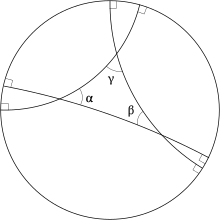
\includegraphics[width=0.5\textwidth]{assets/hyperbolic_triangle.png}
    \caption{Triangolo iperbolico}
\end{figure}

\subsubsection{Curva piana}

\textbf{Ascissa curvilinea}

